It was necessary to design and implement my own database instead of using one
by the university, as they never responded to Dharini's request for either
access or a dump of the database.

\section{Entity Relationship Diagram}
The database underwent several re-designs and iterations. The current version,
which the underlying MariaDB database is implemented on, is version
\texttt{13.c}. Note that in ER-diagrams the relationship quantifiers are read
opposite to UML-diagrams, i.e. following a path out of a table, the quantifier
relevant to the table is on the side \textit{going into} the relationship, and
\textit{not} on the side coming out of the relationship.
\begin{figure}[H]
    \centering
    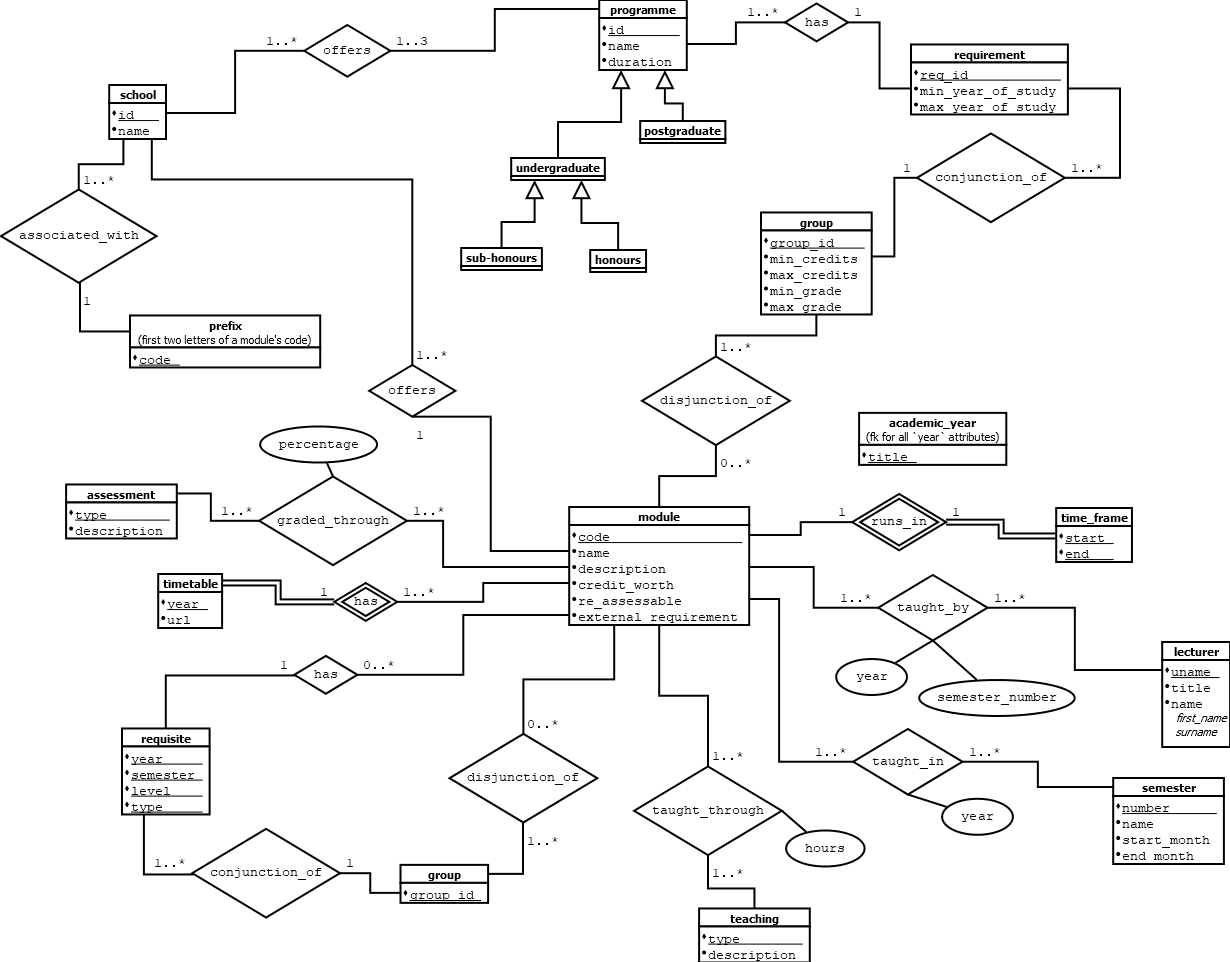
\includegraphics[width=\linewidth]{../Database/ER-Diagram-LATEST.png}
    \caption{The ER-diagram which the underlying database is based upon.}
\end{figure}
Note that two tables cannot have the same name. As such, there are slight
inconsistencies between the names in the ER-diagram and the names used in the
database: the \texttt{group} table used for programme requirements is called
\texttt{disjunctive\_group} and the \texttt{group} table used for module
requisites is called \texttt{requisite\_group}. For the full details, see the
relational model (Appendix \ref{app:rel-model}).

    \subsection{Constants}
    There are 5 tables which contain ``constants''. These are:
    \begin{itemize}
        \item[\texttt{assessment}] Contains the 3 types of assessment that the
              university acknowledges/use on their website. These are: ``Written
              Examination'', ``Practical Examination'', and ``Coursework''. The
              first two entries have a description pulled from the university's
              website. There is no official description for coursework.
        \item[\texttt{semester}] Contains the 4 time periods that a module can
              run in: ``Semester 1'' (numbered 1), ``Semester 2'' (numbered 2),
              ``Summer'' (numbered 3), and ``Whole Year'' (numbered 4).
        \item[\texttt{teaching}] Contains the types of teaching that I was
              able to come up with, it is possible that there are more.
              Currently, the table contains the values ``Lecture'',
              ``Tutorial'', ``Seminar'', ``Supervised laboratory work'',
              ``Field work'', ``Exercise class'', ``Independent study''.
        \item[\texttt{school}] Contains all the schools/departments of the
              university with a numeric ID to quickly identify them. Because
              they also offer modules, the following are also considered
              schools: ``The Music Centre'', ``English Language Teaching'',
              ``The Graduate School''.
        \item[\texttt{prefix}] Contains two letters which uniquely identify what
              school a module is offered by, e.g. modules starting with `CS' are
              offered by the School of Computer Science. This is useful when
              adding modules to the database, as it allows the procedures to
              look up the relevant school given a module code to add, which
              greatly facilitates creating modules by scraping them from the
              university's website. Being able to do this is largely the reason
              why the three `non-schools' are in the \texttt{school} table. The
              inter-disciplinary modules, code `ID', can be offered by any
              school and so do not have an entry in this table.
    \end{itemize}

    \subsection{The \texttt{programme} table and its relationships}
    The \texttt{programme} table contains a unique ID, a name (e.g. ``Bachelor
    of Science (Honours) Computer Science''), a duration (e.g. ``4 years''), and
    a type (``Undergraduate'' or ``Postgraduate''). Looking to the left of the
    table, we can see that a programme is offered by at least 1 and at most 3
    schools, modelling single- to triple-honours. Triple-honours are rare, but
    are offered by some language programmes, e.g. the ``Master of Arts (Honours)
    French, German and Italian'' programme. Going back that path, we can see
    that a school offers at least one programme.
    
    Looking to the right of the \texttt{programme} table, things get a bit more
    complicated. This is due to requirements being expressed in conjunctive
    normal form (CNF), which is tricky to model in a database. A 
    \texttt{programme} has at least one \texttt{requirement} consisting of a
    conjunction of at least one \texttt{group} which itself consists of a
    disjunction of at least one \texttt{module}. This `chain' of tables models
    CNF in the following way: each \texttt{group} represents a compulsory part
    which must be fulfilled to satisfy the \texttt{requirement}; each
    \texttt{module} in the group then represents several options of which
    \textit{at least one} must be taken to fulfill the \texttt{group}
    sub-requirement. Written out in pseudo-logic, it could look as follows:\\
    \begin{math}
        requisite := (module_{a1} \lor module_{a2} \lor ... \lor module_{an})
        \land\ ...\ \land (module_{z1} \lor ... \lor module_{zm})
    \end{math}
    \\
    
    Each \texttt{requirement} has a unique ID, and a minimum and maximum year of
    study. The latter is because whilst most STEM-programmes have the yearly
    requirements matching the module-level (e.g. second year means 2000-level
    modules), some other departments (e.g. the School of Philosophy) have
    requirements along the lines of ``\textit{0 to 80 credits from PY1000-PY2000
    level modules across first and second year}''. A \texttt{requirement}
    belongs to exactly one \texttt{programme} and contains at least one
    \texttt{group} of modules.
    
    Each \texttt{group} in a \texttt{requirement} has a unique ID, a minimum and
    maximum number of credits, and a minimum and maximum grade to achieve. This
    is to model things similar to the School of Philosophy example given above,
    and also the case where certain programmes require an 11 or higher across
    all modules. A \texttt{group} belongs to exactly one \texttt{requiremnt} and
    contains at least one \texttt{module}. Modules do not have to be part of any
    requirement but can exist as purely optional. As previously stated, modules
    in a \texttt{group} are alternatives to each other, where at least one of
    the modules in the \texttt{group} must be taken. There is bound to be some
    duplication of module-groups across certain programmes. However, this model
    was the best way Dr. Ruth Letham and I could come up with to capture the
    CNF-structure of programme requirements.
    
    \subsection{The \texttt{module} table and its relationships}
    The \texttt{module} table contains a unique code (e.g. ``CS1002''), a name,
    a description, a credit worth, whether the module is re-assessable or not,
    and optionally some external requirements. The external requirements are
    free text, as they are intended for requirements like
    ``\textit{Additionally, you must have mathematics (either higher or A-level)
    at grade A or better}'', which are not a module but still a requirement.
    Since it is rare for modules beyond 1000-level to have these, external
    requirements may be \texttt{NULL}.
    
    Going clockwise, the first table around the \texttt{module} table is the
    \texttt{academic\_year} table. This table is not directly linked to the
    module table, but affects nearly all the attributes/details of a module,
    represented by the other surrounding tables. These may vary from year to
    year, and so instead of duplicating the year across multiple tables, they
    refer to an entry in the \texttt{academic\_year} table. The `\texttt{title}'
    of an academic year is its string-representation, e.g. `2019-2020'. This is
    the way the website refers to academic years and is arguably easier to read,
    and model, than having two primary keys \texttt{start\_year} and
    \texttt{end\_year}.
    
    The next table is the \texttt{time\_frame} table. It represents the duration
    that a module is offered. If this is not known, the \texttt{end} entry could
    be set to 100 years in the future. The idea behind this table was to avoid
    students, or advisers, planning for modules in 2 years time only to then
    find out that the module was due to be discontinued 1 year later. A module
    runs in exactly one time-frame, and each time-frame is associated with
    exactly one module.
    \\
    
    The next three tables are related to the teaching of the module. A module is
    taught at least once, in a year and a semester, by at least one
    \texttt{lecturer}. A \texttt{lecturer} has a user-name (e.g. teh6), a title
    (e.g. `Dr.'), and a name which is composed of a first name and a surname. A
    \texttt{lecturer} teaches at least one module. Each module is also taught
    in at least one \texttt{semester}, which may vary from year to year. A
    \texttt{semester} has a number, a name, and a start and end month. There is
    at least one module per semester per year. The final table related to the
    teaching of a module is the \texttt{teaching} table. A module is taught in
    a certain number of hours, using a certain teaching type, e.g. lectures.
    Each teaching type also has a description, explaining what that teaching
    type is.
    \\
    
    Continuing clockwise, there is a loop of tables. This loop uses the same
    `chaining' of tables used to model programme requirements, to model module
    requisites. Similar to programme requirements, module requisites are
    expressed in CNF: a \texttt{module} may have 0 or more \texttt{requisites},
    each of which consists of at least one \texttt{group}. All the
    \texttt{groups} must be satisfied to satisfy the \texttt{requisite}, and
    each \texttt{group} contains at least one \texttt{module}. If a group
    contains multiple \texttt{module}s, at least one of them must be taken to
    satisfy the \texttt{group} sub-requisite. The main differences to programme
    requirements are that module requisites can vary across academic years,
    semesters, and levels (``UG'', ``PGT'', or ``PGR''), and have a type, i.e.
    ``Pre'', ``Co'', or ``Anti''. A further difference is that the
    \texttt{group} table serves purely to provide a group ID to identify
    alternatives, and that these alternatives are themselves entries in the
    \texttt{module} table. A \texttt{module} does not have to be part of a
    requisite \texttt{group}, but each \texttt{group} must be associated with
    exactly one requisite.
    \\
    
    The final two tables, going clockwise, contain additional information about
    a module. A \texttt{timetable} is identified by its associated
    \texttt{module} and year, but due to timetables not being agreed far in
    advance, I simply store the URL to the timetable information, if exists. If
    the information does not yet exist, the URL is \texttt{NULL}. Finally, each
    module is graded through at least one type of \texttt{assessment}, e.g.
    ``Written Examination''. There is a percentage associated with this, which
    must not be greater than 100\%. A typical distribution for CS-coded modules
    is to have 40\% coursework and 60\% written examination.
    \\
    
    This concludes the various attributes and relationships associated with the
    \texttt{module} table. It turns out modules are fairly complex, but I
    believe the current data-model captures all that is necessary for the
    project, and possibly a bit extra which could be useful for querying about
    details of a specific module.

\section{Views}
There are two views in the database: \texttt{complete\_modules} and
\texttt{complete\_requisites}.

    \subsection{Complete Modules}
    The \texttt{complete\_modules} view displays
    information similar to what can be found on the university's module search 
    with the name of the school offering the module also being displayed.
    Similar to the university's portal, there is an entry per module per taught
    instance, e.g. if a module is taught this year and the next, there will be 2
    entries. This is also true if the module is taught twice per year. The view
    is constructed by joining the \texttt{module} table with the
    \texttt{taught\_in} table, matching on the module codes, and then further
    joining with the \texttt{school} table, matching the module's
    \texttt{school\_id} to the \texttt{id} of the \texttt{school}.

    \subsection{Complete Requisites}
    The \texttt{complete\_requisites} view displays all details of all the
    requisites, i.e. what module has the requisite, what type of requisite it
    is, the disjunctive group IDs, and the modules involved. The view is
    constructed by first joining the \texttt{requisite} table with the
    \texttt{requisite\_group} table, matching the requisite IDs, and then
    joining with the \texttt{disjunctive\_group} table, matching the disjunctive
    group IDs. The resulting view is quite big, as it duplicates rows for each
    requisite, for each alternative in a group. This could potentially be
    improved by only duplicating rows for each group and coalescing all the
    module codes in a group into a list-like structure. The potential
    disadvantage to this, is that it might be more difficult to deal with on the
    machine-readable side of things, e.g. a server.

\section{Procedures}
To facilitate data insertion, and by extension the web scraping, there are
several stored procedures defined in the database:
\begin{itemize}
    \item \texttt{create\_pre\_requisite}
    \item \texttt{add\_alt\_pre\_req\_by\_existing\_pre\_req}
    \item \texttt{create\_co\_requisite}
    \item \texttt{add\_alt\_co\_req\_by\_existing\_co\_req}
    \item \texttt{create\_anti\_requisite}
    \item \texttt{create\_id\_module}
    \item \texttt{create\_prefix\_association}
    \item \texttt{create\_catalogue\_entry}
\end{itemize}
The functionality and details of each of these is explained in this given order
in the sub-sections below.

    \subsection{Creating a pre-requisite}
    To create a pre-requisite, the user must supply a source module code, a
    target module code, the academic level that the requisite applies to, the
    academic year the requisite concerns, and the semester the requisite
    concerns. These arguments must be provided in this order. The
    \textbf{source} module is the module that \textbf{requires} something, and
    the \textbf{target} module is the module that \textbf{is required} by the
    source.
    
    The procedure checks that both the modules exist and, if they do, creates
    a new entry in the \texttt{requisite} table, fetches the newly created
    requisite's auto-incremented ID, uses that ID to create a new entry in the
    \texttt{requisite\_group} table and fetches the new requisite group's
    auto-incremented ID, and then uses \textit{that} ID to create an entry for
    the target module in that group (through the \texttt{disjunctive\_group}
    table). If either the source or the target module does not exist, the
    procedure errors, reporting which module did not exist.
    \\
    
    Each pre-requisite created using this procedure is considered to be
    conjunctive, i.e. each must be satisfied to be able to take the source
    module. To create disjunctions, add alternatives, use the procedure
    described in the next sub-section.
    
    \subsection{Adding an alternative pre-requisite}
    To add an alternative module there must already exist a pre-requisite to add
    it to. An alternative is created by knowing the source (i.e. the module
    which requires the other module(s)) module code; an existing target module
    code, as well as the academic level, academic year, and semester of the
    existing pre-requisite; and finally, the module code of the alternative
    target module.
    
    The procedure checks that the alternative to add exists and, if it does,
    uses the existing details in combination with the
    \texttt{complete\_requisites} view to find the group ID that the alternative
    should be added to, and then adds it to the group with that ID (through the
    \texttt{disjunctive\_group} table). If the alternative module does not exist
    or there is no group matching the given details of the supposedly existing
    requisite, the procedure errors, reporting what went wrong.
    \\
    
    Modules added using this procedure are considered alternatives, i.e. at
    least one of them must be taken to satisfy the group requirement. To add
    another module which must \textit{also} be taken, use the procedure
    described in the previous sub-section.
    
    \subsection{Creating a co-requisite}
    To create a co-requisite, the user must supply the same arguments as for
    creating a pre-requisite, i.e. a source module code, a target module code,
    the academic level that the requisite applies to, the academic year that the
    requisite concerns, and the semester the requisite concerns. The procedure
    checks that both the modules exist and, if they do, creates the co-requisite
    through the same steps as creating a pre-requisite. If either the source or
    the target module does not exist, the procedure errors, reporting which
    module did not exist.
    \\
    
    Each co-requisite created using this procedure is considered to be
    conjunctive, i.e. each target must be taken along with the source module if
    one is to do the source module. To create disjunctions, add alternatives,
    use the procedure described in the next sub-section.
    
    
    \subsection{Adding an alternative co-requisite}
    To add an alternative module as a co-requisite, there must already exist a
    co-requisite to add it to. An alternative is created by knowing the same
    parameters as for adding an alternative pre-requisite, i.e. an existing
    source module code; an existing target module code; the academic level,
    academic year, and semester of the existing co-requisite; and the module
    code of the alternative target module. The procedure uses the same steps as
    the procedure for adding alternative pre-requisites, with the only
    difference being modifying requisites of \texttt{type} `Co'. If the
    alternative module does not exist or there is no group matching the given
    details of the supposedly existing requisite, the procedure errors,
    reporting what went wrong.
    \\
    
    Modules added using this procedure are considered alternatives, i.e. at
    least one of them must be taken along with the requiring/source module if
    one wants to take the source module. To add another module which must
    \texttt{also} be taken along with the source module, use the procedure
    described in the previous sub-section.
    
    \subsection{Creating an anti-requisite}
    To create an anti-requsitie, the user must supply the same arguments as for
    creating a pre-requisite or a co-requisite, i.e. a source module code, a
    target module code, the academic level that the requisite applies to, the
    academic year that the requisite concerns, and the semester the requisite
    concerns. The procedure checks that both the modules exist and, if they do,
    creates \textbf{two (2)} anti-requisites: one from source to target, and one
    from target to source. Each anti-requisite is created using the same steps
    used to create a pre-requisite. Creating the requisites both ways guarantees
    that no-one can accidentally be advised onto a module they had an
    anti-requisite for due to someone forgetting to add the record of the
    anti-requisite on the other side. If either the source or the target module
    does not exist, or there already exists an anti-requisite with all the given
    specifics in either direction, then the procedure errors, reporting what
    went wrong.
    \\
    
    There is no option to add an alternative anti-requisite as it does not make
    sense to think/talk about alternative anti-requisites; All anti-requisites
    are conjunctive. This can also be reasoned about by looking at the logic
    representation:
    \\
    $\lnot (a \lor b)$ is the same as $\lnot a \land \lnot b$
    
    \subsection{Creating an ID module}
    To create an interdisciplinary (ID) module, the user must supply the name of
    the school offering the module, the module code, the module name, the
    academic year the module runs in, the module's SCOTCAT credit worth, the
    number of the semester the module runs in, the module description, and a
    boolean indicating whether the module can be re-assessed/re-sat or not.
    
    The procedure checks that the module is ID-coded and that there is a school
    with the given name. If either is not the case, the procedure errors,
    reporting what went wrong. If everything is okay, the procedure inserts the
    academic year in the \texttt{academic\_year} table unless it is already
    present, finds the school ID based on its name, creates the module, and
    creates an entry in the \texttt{taught\_in} table. This ensures the
    academic year exists and that the module is taught at least once. Using the
    school name to look up the ID helps prevent the user potentially
    misremembering or mis-typing the school ID as names are easier to remember.
    
    \subsection{Creating a prefix association}
    To create a prefix association, the user must supply the prefix (e.g. `CS')
    and the name of the school to associate it with (e.g. `School of Computer
    Science'). Since all schools will have some prefix associated with them,
    if this procedure is called with a non-existant school, the school will be
    created. If the school already exists, it will not. In either case, the ID
    of the school is found, and used to create an entry in the
    \texttt{prefix\_association} table. Schools can be associated with multiple
    prefixes, but each prefix should match exactly one school.
    
    \subsection{Creating a catalogue entry}
    A catalogue entry is defined as the information that comes up when searching
    on the university's catalogue portal, with the exception of requisites and
    external requirements, as these would require the procedure to support
    variadic arguments. This procedure relies on the entries in the
    \texttt{prefix\_association} table and therefore should never be used with
    ID-coded modules, as they cannot be uniquely mapped to a school.
    \\
        
    To create a catalogue entry, the user must supply the
    module code, the module name, the academic year the module is taught in, the
    module's SCOTCAT credit worth, the number of the semester in which the
    module is taught, the module description, and a boolean indicating whether
    the module can be re-assessed/re-sat or not.
    
    The procedure creates the academic year if it does not already exist, uses
    the \texttt{prefix\_association} table to look up the school offering the
    module based on the first two characters in the code, creates the module if
    it does not already exist, and creates a \texttt{taught\_in} entry for the
    relevant academic year and semester. Attempting to re-create an existing
    module with different semester and academic year inputs will succeed by
    creating an entry in the \texttt{taught\_in} table, but this will also warn
    that the module already existed.

\section{Web Scrapers for Data Population}
I initially thought of entering the data manually. This might have been fine for
just the Computer Science modules, although it probably would have taken at
least a day of very repetitive work. The number of modules for CS is not that
many. The problem arises from the fact that the website has a row for each year
and semester that a module is taught, often resulting in 2 or 4 entries for the
same module (the website only shows the current academic year and the previous).
Alice Lynch wrote a web-scraper in Python, based on the data I thought I needed.
I then modified this scraper to include the SQL-queries, and to parse and split
the strings to extract the necessary information. This resulted in 3 scrapers:
\begin{itemize}
    \item \texttt{module-magic.py}
    \item \texttt{prefix-magic.py}
    \item \texttt{requisite-magic.py}
\end{itemize}

The `\texttt{magic}' part of the name is because the scrapers are highly
specialised and use a lot of magic regular-expressions and string-splitting.
They can be used to scrape one thing from one website, and nothing more. If
something else needs scraping, it would be better to copy and modify the
original scraper rather than try to extend any of the existing ones. Each
scraper takes some arguments and flags. The details of these can be found by
passing the \texttt{-h} or \texttt{--help} flag when calling them.
\\

Common to all the scrapers is that they print the SQL-queries that will be
executed and asks the user to confirm them. \textbf{It is highly recommended} to
skim over all of these to sanity-check that none of the scraped pages contained
some oddity not previously encountered. This happened on several occasions when
I was using them, so whilst some oddities have been caught and adapted to, it is
still likely that there might be others.

    \subsection{Prefix scraper}
    The prefix scraper was used to scrape the schools and the various
    module-code prefixes associated with them. This was done by constructing a
    dictionary mapping prefixes to school names. The key-value pairs are then
    stored in the database using the \texttt{create\_prefix\_association}
    procedure.
    
    It is unlikely that this scraper has to be used more than once as it scrapes
    all the prefixes rather than a specific subset.

    \subsection{Module scraper}
    The module scraper takes a prefix/school code and scrapes all the modules
    matching that prefix. Since the table-view of the website has duplicate
    entries for modules taught in both semesters, compared to the page for the
    module which says ``\texttt{Semesters: BOTH}'', the semester number is
    scraped from this table. The remaining details, i.e. the module code,
    module name, academic year, SCOTCAT credit worth, module description, and
    whether the module is re-assessable, are all scraped from the catalogue
    page.
    \\
    
    There are a couple of features useful for testing and debugging:
    \begin{itemize}
        \item The number of modules scraped can be limited by passing the
              \texttt{-l} or \texttt{--limit} flag followed by an integer.
        \item Passing in a module code or a prefix followed by a number (e.g.
              `\texttt{CS3}') will work and only scrape that specific module or
              the modules at that level respectively.
    \end{itemize}
    
    \subsection{Requisite scraper}
    The requisite scraper takes a prefix and scrapes all the requisites of all
    the modules matching that prefix. This scraper is the largest and messiest
    because of the vast number of inconsistencies across the website. A few
    examples are: Undergraduate requisites can be denoted by the word
    `Undergraduate', the abbreviation `UG', or the abbreviation `Ug', and
    similar for postgraduate requisites (`PGT'); which notation is used is
    usually consistent in the same description, i.e. both undergraduate and
    postgraduate requirements are referred to by the capitalised abbreviation,
    except for when it isn't; undergraduate requirements come before the
    postgraduate requirements, except for when they don't; it is usually only
    5000-/masters-level modules that have co-requisites, except for when it
    isn't; etc... All of these edge-cases lead to a number of magic regular
    expressions, string-matching, and string-splitting. The current version
    seems to work, but it may be the case that when more schools' modules are
    scraped (beyond just CS and Biology), more edge cases will pop up. These
    will then have to be added to the scraper.
    \\
    
    The scraper starts by grouping the pre-, co-, and anti-requisites for each
    module, for each semester and academic year. If a module has no requisites
    of a certain type, the variable the group would be stored in is
    \texttt{None}. Each of these groups is then split into `levels', i.e.
    undergraduate or postgraduate, using a large number of \texttt{if-else}
    statements, regular expressions, and substring-matching. Finally, each of
    the undergraduate and postgraduate, pre-, co-, and anti-requisites are
    committed to the database using the appropriate stored procedures. The
    scraper takes alternatives into account, calling the stored procedures to
    create alternative requisites as appropriate.
